\subsection{Đề 3}
\Opensolutionfile{ans}[ans/ans-2-OTGK1-De3-LC]
\caulc

\begin{ex}%[2D1N1-2]
	Cho hàm số $f(x)$ có bảng biến thiên như sau
	\begin{center}
		
\begin{tikzpicture}[>=stealth,thick]
			\tkzTabInit[nocadre,lgt=1.2,espcl=2,deltacl=0.5]{$x$/.7 ,$f'(x)$/.7,$f(x)$/2}
			{$-\infty$ , $-1$ , $0$ , $1$ , $+\infty$}
			\tkzTabLine{ , - , $0$ , + , $0$ , - , $0$ , + , }
			\tkzTabVar{+/$+\infty$ , -/$-1$, +/$4$ , -/$-1$ , +/$+\infty$}
		\end{tikzpicture}
	\end{center}
	Hàm số đã cho đồng biến trên khoảng nào dưới đây?
	\choice
	{$\left(-\infty ;-1\right)$}
	{$\left(0;1\right)$}
	{$\left(-1;1\right)$}
	{\True $\left(-1;0\right)$}
	\loigiai{
		Hàm số đã cho đồng biến trên khoảng $\left(-1;0\right)$ và $\left(1;+\infty\right)$.}
\end{ex}

\begin{ex}%[2D1V2-3]
	Tìm giá trị thực của tham số $m$ để hàm số $y=\dfrac{1}{3}{x^3}-m{x^2}+\left(m^2-4\right)x+3$ đạt cực trị tại $x=3$.
	\choice
	{$m=-1$; $m=-7$}
	{$m=-7$}
	{\True $m=5$; $m=1$}
	{$m=5$}
	\loigiai{
		Ta có $y'=x^2-2mx+\left(m^2-4\right)$.\\
		Hàm số $y=\dfrac{1}{3}{x^3}-m{x^2}+\left(m^2-4\right)x+3$ đạt cực trị tại $x=3$ khi và chỉ khi $$y'(3)=0\Leftrightarrow 9-6m+m^2-4=0 \Leftrightarrow m^2-6m+5=0\Leftrightarrow \hoac{&m=1\\&m=5.}$$
		Vậy $m=5$; $m=1$ là giá trị cần tìm.
	}
\end{ex}

\begin{ex}%[2D1N3-1]
	\immini{
		Cho hàm số $y=f(x)$ liên tục trên đoạn $[-1;3]$ và có đồ thị như hình bên. Gọi $M$ và $m$ lần lượt là giá trị lớn nhất và giá trị nhỏ nhất của hàm số đã cho trên đoạn $[-1;3]$. Giá trị của $M-m$ bằng
		\choice
		{$1$}
		{$4$}
		{\True $5$}
		{$0$}
	}{
		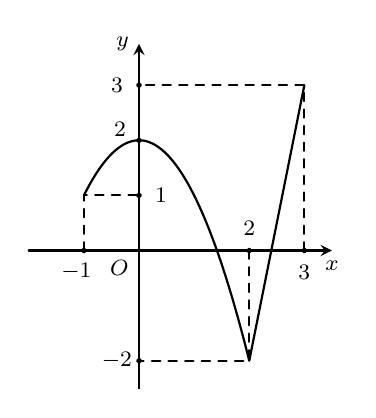
\begin{tikzpicture}[>=stealth,line join=round,line cap=round,font=\footnotesize,scale=0.7,thick]
			\draw[->] (-2,0)--(3.5,0) node[below]{$x$};
			\draw[->] (0,-2.5)--(0,3.75) node[left]{$y$};
			\fill[name=O] (0,0) circle (1pt) node[below left] {$O$}; 
			\draw[thick,color=black, smooth, samples=100, domain= -1:2] plot(\x,{-(\x)^2 +2}) node[left]{$ $};
			\draw[thick] (2,-2)--(3,3);
			\draw[dashed] (-1,0)|-(0,1) (2,0)|-(0,-2) (3,0)|-(0,3);
			\foreach \d/\g/\l in {{-1,0}/-110/-1,{2,0}/90/2,{3,0}/-90/3,{0,-2}/180/-2,{0,1}/0/1,{0,2}/150/2,{0,3}/180/3}
			\draw[fill=black] (\d) circle (1pt) +(\g:.4) node{$\l$};
		\end{tikzpicture}
	}
	\loigiai{
		Từ đồ thị, ta có $M=\max\limits_{[-1;3]}f(x)=3$ và $m=\min\limits_{[-1;3]}f(x)=-2$.\\
		Vậy $M-m=5$.
	}
\end{ex}

\begin{ex}%[2D1N3-1]
	Xét hàm số $y=f(x)$ với $x\in [-1;5]$ có bảng biến thiên như sau
	\begin{center}
		
\begin{tikzpicture}
			\tkzTabInit[nocadre=false,lgt=1.2,espcl=2.3,deltacl=.6]
			{$x$/0.6,$y'$/0.6,$y$/2}
			{$-1$,$0$,$2$,$5$}
			\tkzTabLine{,+,0,-,0,+,}
			\tkzTabVar{-/$3$,+/$4$,-/$0$,+/$+\infty$}
		\end{tikzpicture}
	\end{center}
	Khẳng định nào sau đây đúng?
	\choice
	{\True Hàm số đã cho không tồn tại giá trị lớn nhất trên đoạn $[-1;5]$}
	{Hàm số đã cho đạt giá trị nhỏ nhất tại $x=-1$ và $x=2$ trên đoạn $[-1;5]$}
	{Hàm số đã cho đạt giá trị nhỏ nhất tại $x=-1$ và đạt giá trị lớn nhất tại $x=-5$ trên đoạn $[-1;5]$}
	{Hàm số đã cho đạt giá trị nhỏ nhất tại $x=0$ trên đoạn $[-1;5]$}
	\loigiai{
		Từ bảng biến thiên, ta có hàm số không tồn tại giá trị lớn nhất trên đoạn $[-1;5]$.
	}
\end{ex}

\begin{ex}%[2D1N4-1]
	Cho hàm số $y=f(x)$ có $\lim\limits_{x\rightarrow +\infty}y=1$ và $\lim\limits_{x\rightarrow -\infty}y=-1$. Khẳng định nào sau đây là khẳng định đúng?
	\choice
	{Đồ thị hàm số đã cho không có tiệm cận ngang}
	{Đồ thị hàm số đã cho có đúng một tiệm cận ngang}
	{\True Đồ thị hàm số đã cho có hai tiệm cận ngang là các đường thẳng $y=1$ và $y=-1$}
	{Đồ thị hàm số đã cho có hai tiệm cận ngang là các đường thẳng $x=1$ và $x=-1$}
	\loigiai{
		Theo định nghĩa đường tiệm cận, ta có
		\begin{itemize}
			\item $\lim\limits_{x\rightarrow +\infty}y=1$ suy ra $ y=1 $ là đường tiệm cận ngang.
			\item $\lim\limits_{x\rightarrow -\infty}y=-1$ suy ra $ y=-1 $ là đường tiệm cận ngang.
		\end{itemize}
	}
\end{ex}

\begin{ex}%[2D1V4-1]
	Tổng số tiệm cận đứng và tiệm cận ngang của đồ thị hàm số $ y=\dfrac{5x^2-4x-1}{x^2-1} $ là 
	\choice
	{$ 0 $}
	{$ 1 $}
	{\True $ 2 $}
	{$ 3 $}
	\loigiai
	{
		Hàm số xác định khi $x \ne \pm 1$.
		\begin{itemize}
			\item Tiệm cận ngang:
			\[\lim \limits_{x \to \pm\infty} y = \lim \limits_{x \to \pm \infty} \dfrac{5x^2-4x-1}{x^2-1} = \lim \limits_{x \to \pm \infty} \dfrac{5-\dfrac{4}{x}-\dfrac{1}{x^2}}{1-\dfrac{1}{x^2}}=5.\]
			Suy ra đồ thị hàm số có một tiệm cận ngang $ y=5 $.
			\item Tiệm cận đứng:
			Cho $x^2=1 \Leftrightarrow \hoac{&x=1\\&x=-1}$
			\[\lim \limits_{x \to 1} y=\lim \limits_{x \to 1} \dfrac{5x^2-4x-1}{x^2-1} = \lim \limits_{x \to 1} \dfrac{(5x+1)(x-1)}{(x+1)(x-1)}=\lim \limits_{x \to 1} \dfrac{5x+1}{x+1}=3.\]
			Suy ra đường thẳng $ x=1 $ không phải là tiệm cận đứng của đồ thị hàm số.
			\[\lim \limits_{x \to -1^{+}} y=\lim \limits_{x \to -1^{+}} \dfrac{5x^2-4x-1}{x^2-1} = \lim \limits_{x \to -1^{+}} \dfrac{1}{x+1} \cdot \dfrac{5x^2-4x-1}{x-1}=-\infty \]
			Vì $\lim \limits_{x \to -1^{+}} \dfrac{1}{x+1} =+\infty$ và $\lim \limits_{x \to -1^{+}}\dfrac{5x^2-4x-1}{x-1} =-4<0$.\\
			Suy ra đồ thị hàm số có một tiệm cận đứng $ x=-1 $.
		\end{itemize}
		Tổng cộng đồ thị hàm số có tổng số tiệm cận đứng và tiệm cận ngang là 2.
	}
\end{ex}

\begin{ex}%[2D1N5-1]
	\immini{
		Đồ thị của hàm số dưới đây có dạng như đường cong bên?
		\choice
		{\True $y=x^3-3x+1$}
		{$y=x^4-2x^2+1$}
		{$y=-x^4+2x^2+1$}
		{$y=-x^3+3x+1$}
	}{
		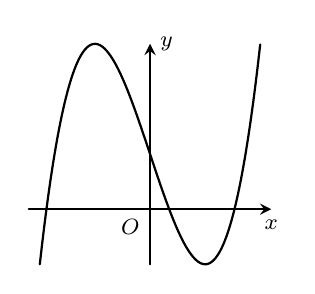
\begin{tikzpicture}[line cap=round, line join=round, font=\footnotesize, >=stealth, scale=0.7,thick]
			\tikzset{label style/.style={font=\footnotesize}}
			\draw[->] (-2.2,0)--(2.2,0) node[below]{$x$};
			\draw[->] (0,-1)--(0,3) node[right]{$y$};
			\draw[smooth, samples=100] plot[domain=-2:2] (\x, {(\x)^3-3*(\x)+1});
			\node at (0,0)[below left]{$O$}; 
		\end{tikzpicture}
	}	
	\loigiai{
		Đồ thị đã cho là đồ thị hàm bậc ba, với hệ số $a>0$.
	}
\end{ex}

\begin{ex}%[2D1N5-1]
	\immini{
		Đồ thị của hàm số nào dưới đây có dạng như đường cong trong dưới đây?
		\choice
		{\True $ y=-x^4+2x^2$}
		{$ y=x^4-2x^2$}
		{$ y=x^3-3x^2$}
		{$ y=-x^3+3x^2$}
	}{
		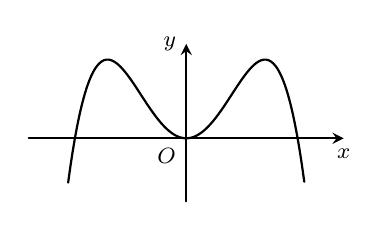
\begin{tikzpicture}[line cap=round, line join=round, font=\footnotesize, >=stealth, scale=1,thick]
			\tikzset{label style/.style={font=\footnotesize}}
			\draw[->] (-2,0)--(2,0) node[below]{$x$};
			\draw[->] (0,-0.8)--(0,1.2) node[left]{$y$};
			\draw[smooth, samples=100] plot[domain=-1.5:1.5] (\x, {-(\x)^4+2*(\x)^2});
			\node at (0,0)[below left]{$O$};
		\end{tikzpicture}	
	}
	\loigiai{
		Từ hình dạng của đồ thị ta loại phương án $ y=x^3-3x^2$ và $ y=-x^3+3x^2$.\\
		Nhận thấy $\lim\limits_{x\to\pm\infty}f(x)=-\infty $ suy ra hệ số của $x^4$ âm nên chọn phương án $ y=-x^4+2x^2$.}
\end{ex}

\begin{ex}%[2D1H5-1]
	Hàm số nào dưới đây có bảng biến thiên như sau:
	\begin{center}
		
\begin{tikzpicture}[thick]
			\tkzTabInit[espcl=2.5,lgt=1.5,nocadre]
			{$x$/0.7,$y'$/0.7,$y$/2.1}
			{$-\infty$,$-1$,$1$,$+\infty$}
			\tkzTabLine{,-,0,+,0,-,}
			\tkzTabVar{+/$+\infty$,-/$-2$,+/$2$,-/$-\infty$}
		\end{tikzpicture}
	\end{center}
	\choice
	{$y=x^3-3x$}
	{$y=x^2-2x$}
	{\True $y=-x^3+3x$}
	{$y=-x^2+2x$}	
	\loigiai{
		Dựa vào bảng biến thiên trên, ta nhận thấy đây là hàm số bậc ba có dạng $y=ax^3+bx^2+cx+d$ với $a\neq 0$.\\
		Mà $\lim\limits_{x\to+\infty}\left(ax^3+bx^2+cx+d\right)=-\infty\Rightarrow a<0$.\\
		Do đó có duy nhất hàm số $y=-x^3+3x$ thoả mãn.}
\end{ex}

\begin{ex}%[2D1N5-8]
	Giả sử chi phí (tính bằng trăm nghìn đồng) để sản xuất $x$ đơn vị hàng hóa nào đó là $C(x)=23000+50x-0{,}5x^2+0{,}00175x^3$. Tìm hàm chi phí biên.
	\choice
	{\True $y=\dfrac{21}{4000}x^2-x+50$}
	{$y=0{,}00175x^2-0{,}5x+50$}
	{$y=\dfrac{21}{4000}x^2-x+23050$}
	{$y=0{,}00175x^2-0{,}5x+23050$}
	\loigiai{
		Hàm chi phí biên là $y=C'(x)=\dfrac{21}{4000}x^2-x+50$.
	}
\end{ex}	

\begin{ex}%[2D1N5-8]
	Khi máu di chuyển từ tim qua các động mạch chính rồi đến các mao mạch và quay trở lại qua các tĩnh mạch, huyết áp tâm thu (tức là áp lực của máu lên động mạch khi tim co bóp) liên tục giảm xuống. Giả sử một người có huyết áp tâm thu $P$ (tính bằng mmHg) được cho bởi hàm số $P(t)=\dfrac{25t^2+125}{t^2+1}$, $0\le t	\le 10$, trong đó thời gian $t$ được tính bằng giây. Tính tốc độ thay đổi của huyết áp sau $5$ giây kể từ khi máu rời tim.
	\choice
	{Tăng $\dfrac{250}{169}$}
	{Tăng $\dfrac{375}{13}$}
	{\True Giảm $\dfrac{250}{169}$}
	{Giảm $\dfrac{500}{13}$}
	\loigiai{
		Tốc độ thay đổi của huyết áp sau $t$ giây là $$P'(t)=\dfrac{50t(t^2+1)-2t(25t^2+125)}{(t^2+1)^2}=-\dfrac{200t}{(t^2+1)^2}.$$
		Suy ra $P'(5)=-\dfrac{200\cdot 5}{(5^2+1)^2}=-\dfrac{250}{169}$.\\
		Tốc độ thay đổi của huyết áp sau $5$ giây kể từ khi máu rời tim là giảm $\dfrac{250}{169}$.
	}
\end{ex}

\begin{ex}%[2D1H5-8]
	Người quản lí của một khu chung cư có $100$ căn hộ cho thuê nhận thấy rằng tất cả các căn hộ sẽ có người thuê nếu giá thuê một căn hộ là $8$ triệu đồng một tháng. Một cuộc khảo sát thị trường cho thấy rằng, trung bình cứ mỗi lần tăng giá thuê căn hộ thêm $100$ nghìn đồng thì sẽ có thêm một căn hộ bị bỏ trống. Người quản lí nên đặt giá thuê mỗi căn hộ là bao nhiêu để doanh thu là lớn nhất?
	\choice
	{$10000000$}
	{$810000000$}
	{\True $9000000$}
	{$800000000$}
	\loigiai{
		Gọi $x$ là số lần tăng giá ($0<x<100$).\\
		Mỗi lần tăng giá thì số căn hộ cho thuê là $100-x$ (căn).\\
		Số tiền thuê căn hộ sau mỗi lần tăng là $8000000+100000x$.\\
		Khi đó tổng số tiền cho thuê căn hộ 1 tháng là
		\allowdisplaybreaks
		\begin{eqnarray*}
			y&=&(8000000+100000x)(100-x)\\
			&=&800000000-8000000x+10000000x-100000x^2\\
			&=&800000000+2000000x-100000x^2.
		\end{eqnarray*}
		Bài toán trở thành tìm $x$ để $y$ lớn nhất\\
		Ta có $y'=-200000x+2000000=0\Leftrightarrow x=10$.\\
		Bảng biến thiên
		\begin{center}
			\begin{tikzpicture}[yscale=.8,xscale=1.5,]
				\begin{scope}[shift={(-.5,.5)}]
					\draw
					%			(0,0) rectangle +(8,-5) 
					(0,-1)--+(0:8) (0,-2)--+(0:8) (1,0)--+(-90:5);
				\end{scope}
				\path
				(0,0) node{$x$}          % <<< dòng 1
				++(0:1.5) node{$0$}
				++(0:2.75) node{$10$}
				++(0:2.75) node{$100$}
				(0,-1) node{$y'$}
				++(0:2.8) node{$+$}	  		% <<< dòng 2
				++(0:1.45) node{$0$}
				++(0:1.5) node{$-$}	
				(0,-3)   node{$y$}       % <<< dòng 3
				++(0:1.5) ++(-90:1)  node (A) {$800000000$}
				++(0:2.75) ++(90:2) node (B) {$810000000$}
				++(0:2.75) ++(-90:2) node (C) {$0$};
				\draw[-stealth] (A)--(B);
				\draw[-stealth] (B)--(C);
			\end{tikzpicture}
		\end{center}
		Dựa vào bảng biến thiên ta thấy doanh thu lớn nhất khi người quản lí đặt giá thuê căn hộ là $$8000000+100000 \cdot 10=9000000 \text{ (đồng).}$$
	}
\end{ex}
\Closesolutionfile{ans}
\indapan{3}{ans/ans-2-OTGK1-De3-LC}

\cauds
\Opensolutionfile{ans}[ans/ans-2-OTGK1-De3-DS]
\begin{ex}%[2D1N5-1]
	\immini{Cho hàm số $y=x^3-3x+1$ có đồ thị $(C)$
		\choiceTF
		{\True Tập xác định $\mathscr{D}=\mathbb{R}$}
		{Đồ thị hàm số cắt trục hoành tại $2$ điểm phân biệt}
		{Hàm số đồng biến trên $(-\infty;-1)\cup (1;+\infty)$}
		{\True Đồ thị của hàm số trên có dạng như hình 1}}
	{\begin{tikzpicture}[scale=0.8, font=\footnotesize, line join=round, line cap=round,>=stealth]%<DTools>
			%Gán số liệu.
			\def\xmin{-2};\def\ymin{-2};\def\xmax{2};\def\ymax{4};
			%Gán tọa độ.
			\coordinate (O) at (0,0);
			%Trục Oxy.
			\draw[->] (\xmin,0)--(\xmax,0) node[below]{$x$};
			\draw[->] (0,-1.5)--(0,\ymax) node[left]{$y$};
			\fill (O) node[below left]{$O$} circle(1pt);
			%Giới hạn đồ thị.
			\clip ({\xmin-0.1},{\ymin-0.1}) rectangle ({\xmax+0.1},{\ymax+0.1});
			\foreach \x in {-1}{
				\fill (\x,0) node[below]{$\x$} circle(1pt);
			}
			\foreach \y in {-1}{
				\fill (0,\y) node[left]{$\y$} circle(1pt);
			}
			%Vẽ đồ thị.
			\draw[thick,samples=100] plot[domain=-2:2](\x,{(\x)^3-3*\x+1});
			\draw (1.2,0)node[below]{$1$} (0,2)node[right]{$2$} (0,3)node[right]{$3$} (0,1)node[right]{$1$};
			\draw[dashed] (-1,0)--(-1,3)--(0,3) (1,0)--(1,-1)--(0,-1);
			\draw (0,-1.3)node[below]{$\text{Hình 1}$};
	\end{tikzpicture}}
	\loigiai{
		\begin{itemchoice}
			\itemch Đúng. Tập xác định $\mathscr{D}=\mathbb{R}$.
			\itemch Sai. Xét hàm số $y=x^3-3x+1$ có $y'=3x^3-3=0\Leftrightarrow \hoac{&x=1\\&x=-1.}$\\
			Bảng xét dấu
			\begin{center}
				\begin{tikzpicture}
					\tkzTabInit[nocadre=true,lgt=1.2,espcl=2.5,deltacl=0.6]
					{$x$ /0.6,$y’$ /0.6,$y$ /2}
					{$-\infty$,$-1$,$1$,$+\infty$}
					\tkzTabLine{,+,0,-,0,+,}
					\tkzTabVar{-/$-\infty$,+/$3$,-/$-1$,+/$+\infty$}
					\draw (2,-2.2)--(9,-2.2)node[below]{$y=0$};
				\end{tikzpicture}
			\end{center}
			Dựa vào bảng biến thiên, ta thấy $y=0$ cắt đồ thị hàm số trên tại $3$ điểm phân biệt nên có $3$ nghiệm phân biệt.
			\itemch Sai. Dựa vào bảng biến thiên ta thấy, hàm số đồng biến trên $(-\infty;-1)$ và $(1;+\infty)$.
			\itemch Đúng.
			\begin{itemize}
				\item Tập xác định $\mathscr{D}=\mathbb{R}$.
				\item Tiệm cận: Không có.
				\item Xét hàm số $y=x^3-3x+1$ có $y'=3x^3-3=0\Leftrightarrow \hoac{&x=1\\&x=-1.}$\\
				Bảng xét dấu
				\begin{center}
					
\begin{tikzpicture}
						\tkzTabInit[nocadre=true,lgt=1.2,espcl=2.5,deltacl=0.6]
						{$x$ /0.6,$y’$ /0.6,$y$ /2}
						{$-\infty$,$-1$,$1$,$+\infty$}
						\tkzTabLine{,+,0,-,0,+,}
						\tkzTabVar{-/$-\infty$,+/$3$,-/$-1$,+/$+\infty$}
					\end{tikzpicture}
				\end{center}
				\item Hàm số đạt cực đại tại $x=-1$ và đạt cực tiểu tại $x=1$.
			\end{itemize}
			Do đó, đồ thị hàm số là hình 1.
	\end{itemchoice}}
\end{ex}


\begin{ex}%[2D1H5-4]
	Cho hàm số $y=\dfrac{2x-3}{x-1}$ có đồ thị $(C)$ và đường thẳng $d\colon y=x+m$.
	\choiceTF
	{\True Đồ thị $(C)$ có tâm đối xứng là $(1;2)$}
	{\True Phương trình tiếp tuyến của đồ thị $(C)$ tại $M\left(3;\dfrac{3}{2}\right)$ là $x-4y+3=0$}
	{Với $m=1$ thì đường thẳng $d$ cắt $(C)$ tại hai điểm phân biệt}
	{Với $m<1$ thì $d$ cắt $(C)$ tại hai điểm phân biệt dương}
	\loigiai{
		\begin{itemchoice}
			\itemch Đúng. Đồ thị hàm số $y=\dfrac{2x-3}{x-1}$ có tâm đối xứng là $I\left(\dfrac{1}{1}; \dfrac{2}{1}\right)\Rightarrow I(1;2)$.
			\itemch Đúng. Xét hàm số $y=\dfrac{2x-3}{x-1}$ có đồ thị $(C)$.
			\begin{itemize}
				\item Tập xác định: $\mathscr{D}=\mathbb{R}\setminus \{1\}$.
				\item Ta có $y'=\dfrac{1}{(x-1)^2}$.
				\item Hệ số góc của tiếp tuyến tại $M\left(3;\dfrac{3}{2}\right)$ là $k=\dfrac{1}{(3-1)^2}=\dfrac{1}{4}$.
			\end{itemize}
			Khi đó, phương trình tiếp tuyến của $(C)$ tại $M\left(3;\dfrac{3}{2}\right)$ là\\ $y=\dfrac{1}{4}\cdot (x-3)+\dfrac{3}{2}\Leftrightarrow x-4y+3=0$.
			\itemch Sai. Với $m=1$ thì $d\colon y=x+1$.\\
			Xét phương trình hoành độ giao điểm giữa $(C)$ và $d$
			\begin{eqnarray*}
				& & \dfrac{2x-3}{x-1}=x+1\\
				&\Leftrightarrow&2x-3=(x+1)(x-1)\\
				&\Leftrightarrow& x^2-2x+2=0\, (\text{phương trình vô nghiệm}).
			\end{eqnarray*}
			\itemch Sai. Xét phương trình hoành độ giao điểm giữa $(C)$ và $d$
			\begin{eqnarray*}
				& & \dfrac{2x-3}{x-1}=x+m \quad (\text{Điều kiện:}\, x\ne 1)\\
				&\Leftrightarrow& 2x-3=(x+m)(x-1)\\
				&\Leftrightarrow& 2x-3=x^2-x+mx-m\\
				&\Leftrightarrow& x^2+(m-3)x-m+3=0\quad (*).
			\end{eqnarray*}
			Để $d$ cắt $(C)$ tại hai điểm phân biệt dương khi và chỉ khi phương trình (*) có hai nghiệm phân biệt dương và khác $1$.
			\begin{align*}
				\Leftrightarrow&\heva{&\Delta>0\\&S>0\\&P>0\\&1^2+(m-3)\cdot 1-m+3\ne0}
				\Leftrightarrow&\heva{&(m-3)^2-4\cdot (-m+3)>0\\&-(m-3)>0\\&-m+3>0}\Leftrightarrow \heva{&m^2-2m-3>0\\&m<3}\\\Leftrightarrow& \heva{&\hoac{&m>3\\&m<-1}\\&m<3}\Leftrightarrow m<-1.
			\end{align*}
		\end{itemchoice}
	}
\end{ex}

\begin{ex}%[2D1H3-6]
	Người ta bơm xăng vào bình xăng của một xe ô tô. Biết rằng thể tích $V$ (lít) của lượng xăng trong bình xăng tính theo thời gian bơm xăng $t$ (phút), sau $30$ giây thì đầy bình. Công thức xác định lượng xăng được đổ vào trong thời gian $t$ là $$V(t)=300(t^2-t^3)+4 \text{ với } 0\le t\le 0{,}5.$$
	\begin{flushright}
		\textit{(Nguồn: R.I. Charles et al., Algebra 2, Pearson)}
	\end{flushright}
	\choiceTF
	{\True Ban đầu trong bình xăng có $4$ lít xăng}
	{\True Lượng xăng có trong bình xăng sau $12$ giây là $13{,}6$ lít}
	{Dung tích của bình xăng trong xe là $45$ lít}
	{Khi xăng chảy vào bình xăng, gọi $V(t)$ là tốc độ tăng thể tích tại thời điểm $t$ với $0\le t\le 0{,}5$. Xăng chảy vào bình xăng ở thời điểm $15$ giây có tốc độ tăng thể tích là lớn nhất}
	\loigiai{
		\begin{itemchoice}
			\itemch Đúng. Số xăng trong bình ban đầu là $V(0)=4$ lít.
			\itemch Đúng. Lượng xăng trong bình xăng sau $12$ giây là\\ $V(0{,}2)=300(0{,}2^2-0{,}2^3)+4=13{,}6$ lít.
			\itemch Sai. Dung tích bình xăng $V=V\left(\dfrac{1}{2}\right)=41{,}5$ lít.
			\itemch Sai. Xét hàm số $V(t)=300(t^2-t^3)+4 \text{ với } 0\le t\le 0{,}5.$\\
			Đạo hàm $V'(t)=300t(2-3t)$.\\
			Cho $V'(t)=0 \Leftrightarrow 300t(t-3t)=0 \Leftrightarrow \hoac{&t=0\in[0;0{,}5]\\&t=\dfrac{2}{3}\notin[0;0{,5}].}$\\
			Các giá trị $V(0)=4$, $V\left(\dfrac{1}{2}\right)=41{,}5$.\\
			Xăng chảy vào bình xăng vào thời điểm ở giây thứ $30$ có tốc độ tăng thể tích là lớn nhất.
	\end{itemchoice}}
\end{ex}


\begin{ex}%[2D1V1-3]
	Cho hàm số $y=-\dfrac{1}{3}x^3-mx^2+(2m-3)x-m+2$.
	\choiceTF
	{\True Với $m=1$ thì hàm số nghịch biến trên $\mathbb{R}$}
	{\True Với $m=\dfrac{3}{2}$ thì hàm số đạt cực đại tại $x=0$}
	{Với $0 \leq m\leq 1$ thì hàm số nghịch biến trên $\mathbb{R}$}
	{Với $m\leq -7$ thì hàm số đồng biến trên $(2;3)$}
	\loigiai{ Xét hàm số $y=-\dfrac{1}{3}x^3-mx^2+(2m-3)x-m+2$ có
		\begin{itemize}
			\item Tập xác định $\mathscr{D}=\mathbb{R}$.
			\item Ta có $y'=-x^2-2mx+(2m-3)$.
		\end{itemize}
		\begin{itemchoice}
			\itemch Đúng. Với $m=1$ ta có $y'=-x^2-2x-1=-(x+1)^2\leq 0$.\\
			Suy ra, hàm số nghịch biến trên $\mathbb{R}$.
			\itemch Đúng. Với $m=\dfrac{3}{2}$ ta có $y'=-x^2-3x=0\Leftrightarrow \hoac{&x=0\\&x=-3.}$\\
			Bảng biến thiên
			\begin{center}
				
\begin{tikzpicture}
					\tkzTabInit[nocadre=true,lgt=1.2,espcl=2.5,deltacl=0.6]
					{$x$ /0.6,$y’$ /0.6}
					{$-\infty$,$-3$,$0$,$+\infty$}
					\tkzTabLine{,-,0,+,0,-,}
				\end{tikzpicture}
			\end{center}
			Dựa vào bảng biến thiên, hàm số đạt cực đại tại $x=0$.	
			\itemch Sai. Ta có $y'=-x^2-2mx+(2m-3)$.\\
			Hàm số nghịch biến trên $\mathbb{R}$ khi  $y'\le0$
			\begin{align*}
				\Leftrightarrow& \heva{a&=-1<0\\&\Delta' \le 0}\\\Leftrightarrow& m^2+2m-3\le 0\\\Leftrightarrow& -3\le m \le 1.
			\end{align*}
			\itemch Sai. Ta có $y'=-x^2-2mx+(2m-3)$.\\
			Hàm số đồng biến trên $(2;3)$ khi  $y'\ge 0\; \forall x\in (2;3)$.
			\begin{eqnarray*}
				& &-x^2-2mx+(2m-3)\ge 0\\
				&\Leftrightarrow&2m\le \dfrac{3+x^2}{1-x}\; \forall x\in (2;3).
			\end{eqnarray*}
			Đặt $g(x)=\dfrac{3+x^2}{1-x}$.\\
			Ta có $g'(x)=\dfrac{-x^2+2x+3}{(1-x)^2}>0\;\forall x\in (2;3)$.\\
			Bảng biến thiên
			\begin{center}
				
\begin{tikzpicture}
					\tkzTabInit[nocadre=true,lgt=1.2,espcl=4,deltacl=0.6]
					{$x$ /0.6,$g’(x)$ /0.6,$g(x)$ /2}
					{$2$,$3$}
					\tkzTabLine{,+,}
					\tkzTabVar{-/$-7$,+/$-6$}
				\end{tikzpicture}
			\end{center}
			Do đó, 	$2m\le \dfrac{3+x^2}{1-x}\; \forall x\in (2;3)\Leftrightarrow 2m\le -7\Leftrightarrow m\le \dfrac{-7}{2}$.
		\end{itemchoice}	
	}
\end{ex}

\Closesolutionfile{ans}
\indapan{3}{ans/ans-2-OTGK1-De3-DS}

\Opensolutionfile{ans}[ans/ans-2-OTGK1-De3-KQ]
\caukq
\begin{ex}%[2D1H1-1]
	Biết rằng hàm số $ y=-x^3+3x^2-4$ đồng biến trên khoảng $(a;b)$. Tính $a+b$.
	\shortans{$2$}
	\loigiai{
		Ta có $y'=-3x^2+6x=0\Leftrightarrow\hoac{& x=0\\& x=2.}$
		\begin{center}
			
\begin{tikzpicture}[thick]
				\tkzTabInit[nocadre,lgt=1,espcl=3]{$x$/0.8,$y'$/0.8,$y$/2}{$-\infty$,$0$,$2$,$+\infty$}
				\tkzTabLine{,-,0,+,0,-,}
				\tkzTabVar{+/$+\infty$,-/$-4$,+/$0$,-/$-\infty$}
			\end{tikzpicture}
		\end{center}
		Dựa vào bảng biến thiên thì hàm số đã cho đồng biến trên khoảng $\left(0;2\right)$.\\
		Suy ra, $a=0$, $b=2$.\\
		Khi đó, $a+b=0+2=2$.
	}
\end{ex}

\begin{ex}%[2D1C1-2]
	\immini{
		Cho hàm số $ y=f(x)$, hàm số $f'(x)=x^3+ax^2+bx+c\left(a,b,c\in\mathbb{R}\right)$ có đồ thị như hình vẽ bên. Biết rằng hàm số $ g(x)=f\left(f'(x)\right)$ nghịch biến trên khoảng $\left(0;\dfrac{a}{b}\right)$ với $a$ là số hữu tỉ và $b$ là số nguyên dương. Tính $a^2+b$.}{
		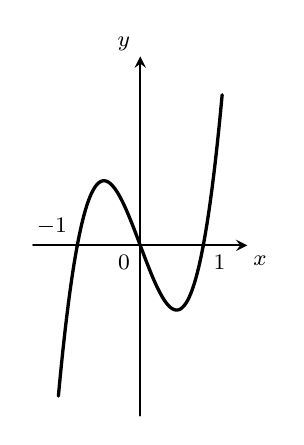
\begin{tikzpicture}[scale=0.8,font=\footnotesize, line join=round, line cap=round, >=stealth,thick] %Đường cong bậc 3
			\draw[thick, ->] (-1.7,0)--(1.7,0);
			\draw[thick, ->] (0,-2.7)--(0,3.0);
			\draw (1.9,0) node[below] {$x$};
			\draw (0,3.2) node[left]{$y$};
			\draw (0,0) node[below left]{$0$};
			\draw[fill] (-1,0) circle (0.5pt)node[above left]{$ -1 $};
			\draw[fill] (1,0) circle (0.5pt)node[below right]{$ 1$};
			\draw[line width=1.2pt,smooth,samples=100,domain=-1.3:1.3] plot(\x,{2.667*(\x)^3+0*(\x)^2-2.667*\x});		
			%\draw[line width=1.2pt,smooth,samples=100,domain=-3.3:2.8] plot(\x,{0.75*(\x)^2+0.5*\x-1});
		\end{tikzpicture}	
	}
	\shortans{$6$}
	\loigiai{	
		Vì các điểm $\left(-1;0\right),\left(0;0\right),\left(1;0\right)$ thuộc đồ thị hàm số $ y=f'(x)$ nên ta có hệ\\
		$\heva{&-1+a-b+c=0\\& c=0\\& 1+a+b+c=0} \Leftrightarrow\heva{& a=0\\ & b=-1\\ & c=0} \Rightarrow {f}'(x)=x^3-x\Rightarrow f''(x)=3x^2-1$.\\
		Ta có $ g(x)=f\left(f'(x)\right)\Rightarrow{g}'(x)=f'\left(f'(x)\right)\cdot f''(x)$.\\
		Xét \\
		$g'(x)=0\Leftrightarrow{g}'(x)=f'\left(f'(x)\right)\cdot f''(x)=0$\\
		$\Leftrightarrow {f}'\left(x^3-x\right)\left(3x^2-1\right)=0\Leftrightarrow\hoac{
			&{x^3}-x=0\\ 
			&{x^3}-x=1\\ 
			&{x^3}-x=-1\\ 
			& 3x^2-1=0} \Leftrightarrow \hoac{
			& x=\pm 1\\ 
			& x=0\\ 
			& x=x_1(x_1\approx 1{,}325)\\ 
			& x=x_2(x_2\approx-1{,}325)\\ 
			& x=\pm\dfrac{\sqrt{3}}{3}.}$\\
		Bảng biến thiên
		\begin{center}
			
\begin{tikzpicture}[thick]
				\tkzTabInit[lgt=1.2,espcl=2,nocadre]
				{$t$/1.0, $h'(x)$ /.7} % first column
				{$-\infty$, $-1{,}325$,$-1$, $-\dfrac{\sqrt{3}}{3}$,$0$,$\dfrac{\sqrt{3}}{3}$,$1$,$1{,}325$, $+\infty$} % first row
				\tkzTabLine { ,-,0,+,0,-,0,+,0,-,0,+,0,-,0,+, } % second row
				%				\tkzTabLine {,-,z,+,t,+,} % third row
				%				\tkzTabLine {,+,d,-,z,+,} % last row
			\end{tikzpicture}
		\end{center}
		Dựa vào bảng biến thiên ta có $g(x)$ nghịch biến trên $\left(0 ;\dfrac{\sqrt 3}{3}\right)$.\\
		Suy ra, $a=\sqrt 3$, $b=3$.\\
		Khi đó $a^2+b=3+3=6$.
	}
\end{ex}

\begin{ex}%[2D1V3-1]
	Có bao nhiêu giá trị của tham số $a$ thuộc đoạn $[-10;10]$ để hàm số $y=ax^4+3x^2+cx$ đạt giá trị nhỏ nhất trên đoạn $[0;4]$ tại $x=1$.
	\shortans{$10$}	
	\loigiai{
		Ta có $f'(x)=4ax^3+6x+c$.\\
		Theo đề bài $y=f(x)=ax^4+3x^2+cx$ đạt giá trị nhỏ nhất trên đoạn $[0;4]$ tại $x=1\Rightarrow f'(1)=0$.\\
		$f'(1)=0\Leftrightarrow 4a+6+x=0\Rightarrow c=-4a-6$.\\
		Khi đó
		\allowdisplaybreaks
		\begin{eqnarray*}
			&&f'(x)=0\\
			&\Leftrightarrow&4ax^3+6x-4a-6=0\\
			&\Leftrightarrow&4a\left(x^3-1\right)+6\left(x-1\right)=0\\
			&\Leftrightarrow&\left(x-1\right)\left[4a\left(x^2+x+1\right)+6\right]=0.
		\end{eqnarray*}
		Để $y=f(x)$ đạt giá trị nhỏ nhất trên đoạn $[0;4]$ tại $x=1$\\
		Suy ra, $4ax^2+4ax+4a+6=0$ vô nghiệm.\\
		Suy ra, $\Delta '=4a^2-4a\left(4a+6\right)<0\Leftrightarrow a^2+2a>0\Leftrightarrow \hoac{&a<-2\\&a>0.}$
		\begin{itemize}
			\item $f(4)>f(1)\Leftrightarrow 256a+48+4\left(-4a-6\right)>a+3+\left(-4a-6\right)\Rightarrow a>\dfrac{-1}{9}$.
			\item $f(0)>f(1)\Leftrightarrow 0>a+3+\left(-4a-6\right)\Rightarrow a>-1$.
		\end{itemize}
		Kết hợp với điều kiện suy ra, $a=\{1;2;3;4;\cdots ;10\}$ hay có $10$ giá trị của $a$ thỏa yêu cầu bài toán.}
\end{ex}

\begin{ex}%[2D1H4-1]
	Cho hàm số $ y=f(x) $ có bảng biến thiên như sau:
	\begin{center}
		
\begin{tikzpicture}[scale=1,thick]
			\tikzset{double style/.append style={double distance=1.5pt}}
			\tkzTabInit[nocadre=false,lgt=1.2,espcl=3.5,deltacl=0.6]
			{$x$ /0.6,$y’$ /0.6,$y$ /2}
			{$-\infty$,$-2$,$+\infty$}
			\tkzTabLine{,-,d,-,}
			\tkzTabVar{+/$-1$,-D+/$-\infty$/$+\infty$,-/$-1$}
		\end{tikzpicture}
	\end{center}
	Tiệm cận ngang của đồ thị hàm số đã cho là đường thẳng có phương trình $y+m=0$. Tìm $m$.
	\shortans{$1$}	
	\loigiai
	{Ta có $ \lim \limits_{x \to \pm \infty}{f(x)}=-1$.\\
		Vậy đồ thị hàm số có tiệm cận ngang là đường thẳng $y=-1 \Leftrightarrow y+1=0$.
	}
\end{ex}

\begin{ex}%[2D1H5-1]
	\immini{
		Cho hàm số $y=ax^3+bx^2+cx+d\left(a,b,c,d\in\mathbb{R}\right)$ có đồ thị là đường cong trong hình bên. Có bao nhiêu số dương trong các số $a$, $b$, $c$, $d$?
	}{
		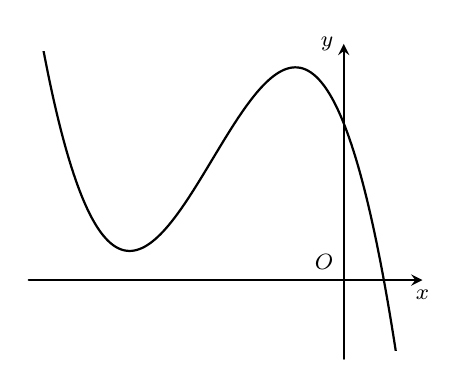
\begin{tikzpicture}[scale=1, font=\footnotesize, line join=round, line cap=round,>=stealth,thick]
			\def\a{-0.5}  % Hệ số co dãn
			\def\xmin{-4} \def\xmax{1}
			\def\ymin{-1} \def\ymax{3} 
			\draw[->] (\xmin,0)--(\xmax,0) node [below]{$x$};
			\draw[->] (0,\ymin)--(0,\ymax) node [left]{$y$};
			\node at (0,0) [above left]{$O$};
			\clip (\xmin+0.1,\ymin+0.1) rectangle (\xmax-0.1,\ymax-0.1);
			\draw[smooth,samples=300] plot(\x,{\a*((\x+3.3)*(\x+2)*(\x-0.3))+1});
		\end{tikzpicture}
	}
	\shortans{$1$}	
	\loigiai{
		Ta có $y'=3ax^2+2bx+c$.\\
		Dựa vào đồ thị ta thấy $a<0$.\\
		Hàm số có $2$ cực trị âm nên $\heva{&\Delta'_{y'}>0\\&S<0\\&P>0}\Leftrightarrow\heva{&b^2-9ac>0\\&-\dfrac{2b}{3a}<0\\&\dfrac{c}{3a}>0}\Rightarrow\heva{&b<0\\&c<0.}$ \\
		Đồ thị cắt trục $Oy$ tại điểm $(0;d)$ nên $d>0$.\\
		Vậy có đúng 1 số dương trong các số $a$, $b$, $c$, $d$.}
\end{ex}

\begin{ex}%[2D1C5-8]
	Một nhà sản xuất trung bình bán được $1000$ ti vi màn hình phẳng mỗi tuần với giá $14$ triệu đồng một chiếc. Một cuộc khảo sát thị trường chỉ ra rằng nếu cứ giảm giá bán $500$ nghìn đồng, số lượng ti vi bán ra sẽ tăng thêm khoảng $100$ ti vi mỗi tuần. Nếu hàm chi phí hằng tuần là $C(x)=12000-3x$ (triệu đồng), trong đó $x$ là số ti vi bán ra trong tuần, nhà sản xuất nên đặt giá bán như thế nào để lợi nhuận là lớn nhất (đơn vị tính: triệu đồng)?
	\shortans{$8$}	
	\loigiai{
		Gọi $p$ (triệu đồng) là giá của mỗi ti vi, $x$ là số ti vi.\\
		Khi đó ta cần xác định hàm cầu $p=p(x)$.\\
		Theo giả thiết tốc độ thay đổi của $x$ tỉ lệ với tốc độ thay đổi của $p$ nên hàm số $p=p(x)$ là hàm số bậc nhất.\\
		Do đó $p(x)=ax+b$ ($a\ne 0$).\\
		Theo đề ta có $x_1=1000$ thì $p_1=14$; $x_2=1100$ thì $p_2=13{,}5$.\\
		Khi đó phương trình đường thẳng $p(x)=ax+b$ đi qua hai điểm $(1000;14)$ và $(1100;13{,}5)$ nên ta có hệ phương trình
		$$\heva{&1000a+b=14\\&1100a+b=13{,}5} \Leftrightarrow \heva{&a=-\dfrac{1}{200}\\&b=19.}$$
		Vậy $p=-\dfrac{1}{200}x+19$.\\
		Khi đó, doanh thu từ bán $x$ ti vi là
		$$R(x)=x\cdot p(x)=x\left(-\dfrac{1}{200}x+19\right)=-\dfrac{1}{200}x^2+19x.$$
		Khi đó tổng lợi nhuận từ bán $x$ ti vi là
		$$P(x)=R(x)-C(x)=-\dfrac{1}{200}x^2+19x-(12000-3x)=-\dfrac{1}{200}x^2+22x-12000.$$
		Bài toán trở thành tìm $x$ để $P(x)$ lớn nhất.\\
		Có $P'(x)=-\dfrac{1}{100}x+22=0\Leftrightarrow -\dfrac{1}{100}x+22=0 \Leftrightarrow x=2200$.\\
		Bảng biến thiên
		\begin{center}
			
\begin{tikzpicture}[thick]
				\tkzTabInit[espcl=4.5,lgt=1.5,nocadre]
				{$x$/0.7,$y'$/0.7,$y$/2.1}
				{$0$,$2200$,$+\infty$}
				\tkzTabLine{,+,0,-,}
				\tkzTabVar{-/$0$,+/$12200$,-/$-\infty$}
			\end{tikzpicture}
		\end{center}
		Dựa vào bảng biến thiên ta thấy số ti vi bán ra trong $1$ tuần là $2200$ chiếc thì lợi nhuận đạt giá trị lớn nhất.\\
		Tức là mỗi tuần bán thêm $1200$ chiếc thì số tiền phải giảm giá $\dfrac{1200 \cdot 500}{100}=6000$ nghìn đồng (tức là $6$ triệu đồng).\\
		Vậy phải để giá bán là $14-6=8$ triệu đồng.
	}
\end{ex}
\Closesolutionfile{ans}
\indapan{6}{ans/ans-2-OTGK1-De3-KQ}